% CS771 final report -- CVPR 2027 author kit, camera-ready mode, 11pt.
% Build (regenerates tables + figures from results/):  bash scripts/build_report.sh
\documentclass[11pt,twocolumn,letterpaper]{article}
\usepackage[T1]{fontenc}       % makes Times (from cvpr.sty) work under XeTeX/tectonic too
\usepackage{cvpr}              % no [review] option => final / camera-ready version
\usepackage{graphicx}
\usepackage{amsmath,amssymb}
\usepackage{booktabs}
\usepackage{xcolor}
\definecolor{cvprblue}{rgb}{0.21,0.49,0.74}
\usepackage[breaklinks,colorlinks,allcolors=cvprblue]{hyperref}
\usepackage{enumitem}
\setlist{nosep,leftmargin=*}
\newcommand{\tbd}[1]{\textcolor{red}{#1}}

\title{Where Occlusion Comes From: Geometric Occlusion Training for\\Skeleton-Based Action Recognition in Smart Homes}
\author{Karthik Reddy Jannupalli \and Sanjana Kallingal \and Penchala Siva Prasanth Kasa\\
University of Wisconsin--Madison}

\begin{document}
\maketitle

%====================================================================
\begin{abstract}
Skeleton-based action recognition is attractive for smart homes because it is light-weight and privacy-preserving,
but home cameras rarely see the whole body: furniture hides the legs and the body hides its own arms.
Robustness is usually trained and tested with \emph{random} joint masking, which does not reflect how occlusion arises.
We replace it with a \emph{geometric} occlusion model, where joints are hidden by ray casting against a virtual
furniture occluder and by projection behind the person's own torso, and hidden joints are corrupted the way a sensor
corrupts them. We test robustness on synthetic structured and held-out occlusions, on \emph{real} Kinect tracking failures in NTU RGB+D,
and on \emph{real homes} (Toyota Smarthome).
Over three seeds, geometric training of ST-GCN is the best or tied-best scheme on every structured occlusion, at no cost in clean accuracy.
On Toyota Smarthome, under added furniture occlusion, it keeps 50.3\% mean-class accuracy against 53.3\% on the unmodified test set; an unaugmented model falls from 53.6\% to 24.6\%.
On real Kinect failures, geometric and random masking each add about $+6$ points.
Combining them is best overall ($+7.0$, and $+10.0$ on heavily occluded clips).
The proposal's lower-body dropout gives almost nothing on real occlusion.
NTU$\rightarrow$Toyota zero-shot transfer is near chance until both datasets share one skeleton normalization.
With it, mean-class accuracy rises from 18--19\% to 22--28\%, and sit down / stand up go from ${\approx}0\%$ to 28--56\%.
\end{abstract}

%====================================================================
\section{Introduction}
Activity recognition in the home, such as detecting a fall, a missed meal or a change in routine, is a central task for ambient assisted living.
3D skeletons from depth sensors~\cite{shotton2011kinect} or RGB pose estimators~\cite{rogez2019lcrnet} make it cheap and privacy-preserving.
Graph networks such as ST-GCN~\cite{yan2018stgcn} recognize actions from them accurately.
These models are usually trained on lab recordings in which the subject is fully visible.
In a real apartment, a table or sofa hides the legs, a person seen from the side or back hides an arm behind the torso, and the sensor responds by guessing or dropping joints (Fig.~\ref{fig:occ}d).

The usual answer is to mask random joints, or a fixed body part, during training and testing~\cite{song2020ragcn}.
Our own proposal did the latter (lower-body dropout).
The two problems with this are the starting point of this project.
First, random masks do not reproduce the \emph{structure} of real occlusion, so they may teach the wrong invariance.
Second, testing with the same random masks says little about real occlusion.

\textbf{Contributions.}
(1)~A geometric occlusion model with three parts: \emph{furniture} (ray casting against a floor-standing box), \emph{self-occlusion} (projection behind the torso) and sensor-style \emph{fill}. It is used as training augmentation and as a test protocol, for both 25-joint Kinect and 13-joint RGB skeletons.
(2)~A four-level evaluation:
(i)~synthetic structured occlusions plus held-out types that no training scheme sees;
(ii)~\emph{real} occlusion from Kinect tracking states on 6{,}043 NTU RGB+D test clips;
(iii)~\emph{real homes}, Toyota Smarthome cross-subject;
(iv)~zero-shot transfer from the lab (NTU) to homes (Toyota).
(3)~Findings, with 3 seeds, on which assumptions about occlusion transfer to real data and which do not (Sec.~\ref{sec:disc}).

%====================================================================
\section{Related Work}
\textbf{Skeleton action recognition.}
ST-GCN~\cite{yan2018stgcn} models the skeleton as a spatio-temporal graph with partitioned graph convolutions.
Later work learns adaptive topologies~\cite{shi2019agcn,chen2021ctrgcn}, and PYSKL~\cite{duan2022pyskl} standardizes training practice.
We use ST-GCN as a representative backbone and keep the backbone fixed, since our question concerns the training signal.

\textbf{Robustness to occlusion.}
RA-GCN~\cite{song2020ragcn} evaluates robustness to dropped body parts and frames and trains extra streams to use non-occluded joints.
Masking-based augmentation is the skeleton analogue of Cutout~\cite{devries2017cutout}.
These approaches remove joints at random or by fixed part, independent of the scene.
Our occlusion model instead derives masks from scene and body geometry, in the spirit of domain randomization~\cite{tobin2017domain}: the occluder is randomized, but its physics is not.

\textbf{Datasets.}
NTU RGB+D~\cite{shahroudy2016ntu} is the standard lab benchmark recorded with Kinect v2.
Toyota Smarthome~\cite{das2019toyota} contains unscripted daily activities of 18 seniors in an apartment, with 7 camera views and heavy furniture occlusion.
Its skeletons come from LCR-Net~\cite{rogez2019lcrnet} applied to RGB.

%====================================================================
\section{Method}
\begin{figure*}[t]
\centering
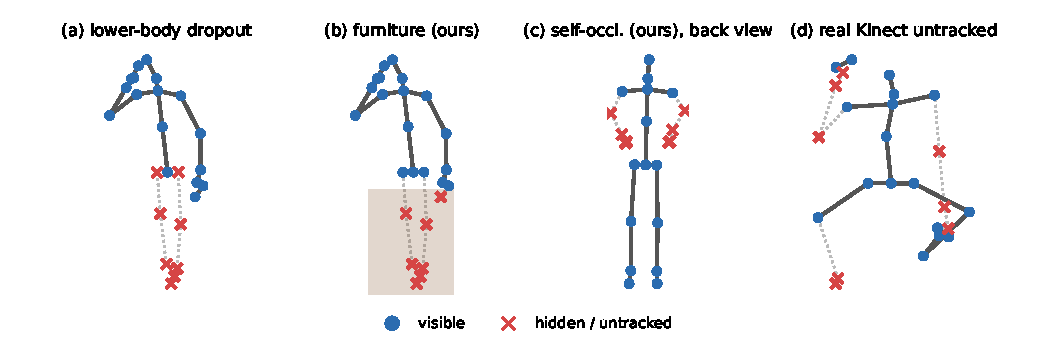
\includegraphics[width=0.92\linewidth]{fig_occlusion.pdf}
\caption{Occlusion on NTU test frames, drawn in the camera image.
(a)~The proposal's lower-body dropout always removes the same eight leg joints.
(b)~Our furniture occluder (brown) hides exactly the joints whose camera ray hits it.
(c)~Our self-occlusion hides the hands behind the torso of a subject facing away.
(d)~A real Kinect frame: untracked joints (red) are mostly hands, wrists and feet, and their reported positions are sensor guesses.}
\label{fig:occ}
\end{figure*}

\textbf{Input.} A clip is $X\in\mathbb{R}^{T\times V\times 3}$ (camera coordinates, $y$ up, $z$ depth), resampled to $T{=}64$ frames.
A visibility mask $M\in\{0,1\}^{T\times V}$ marks occluded joints.
The clip is translated so the center joint(s) (spine-shoulder for NTU, shoulder midpoint for 13 joints) of the first frame where they are \emph{visible} lie at the origin.
Normalization therefore never uses hidden joints. If only one shoulder is visible, it alone is used.

\subsection{Geometric occlusion model}
\textbf{Furniture.}
A box stands on the floor between the camera and the person.
Its front face is the plane $z{=}z_o$, at a random gap of 0.25--0.9\,m in front of the torso.
Its top $y_t$ lies at a random fraction (0.3--1.2) of the foot-to-hip height, and it has a random width (0.35--1.2\,m) and lateral offset.
A joint $p=(x,y,z)$ is hidden when its camera ray crosses the face:
\begin{equation}
z>z_o,\quad y\,\tfrac{z_o}{z}<y_t,\quad \bigl|x\,\tfrac{z_o}{z}-x_c\bigr|<\tfrac{w}{2}.
\end{equation}
Because the box is fixed in space, the mask changes as the person moves (\eg standing up from behind a table).
With probability 0.3 the occluder is present for only part of the clip.

\textbf{Self-occlusion.}
In each frame the torso quadrilateral (shoulders, hips) is projected to normalized image coordinates $(x/z,\,y/z)$ and widened by a body half-thickness of 12\,cm.
A limb joint is hidden if its projection falls inside the torso and it lies more than 4\,cm behind the torso.
This captures arms behind the back, and side and back views, without any learned component.

\textbf{Fill.}
Real sensors rarely output zeros: Kinect reports \emph{inferred} guesses (Fig.~\ref{fig:occ}d).
Hidden joints are therefore either zeroed or held at their last observed position plus 5\,cm Gaussian jitter (``noisy'').

\subsection{Training schemes}
With probability 0.6 per sample, the following are applied:
\begin{itemize}
\item \emph{random}: each joint-frame dropped i.i.d.\ with rate $\mathcal{U}(0.1,0.4)$;
\item \emph{lower-body} (our proposal): all leg joints dropped;
\item \emph{geometric} (ours): furniture (45\%), self-occlusion (25\%), or both (30\%), with zero or noisy fill (50/50);
\item \emph{combined} (ours): geometric masks (75\%), plus sparse sensor-style random dropout ($\mathcal{U}(0.05,0.3)$) on half of those samples and on every remaining sample.
\end{itemize}
None of the schemes ever removes a whole arm or whole frames.
Those two test protocols are therefore held out for all of them.

\subsection{Models and cross-dataset harmonization}
\textbf{Backbones.} ST-GCN~\cite{yan2018stgcn} has 10 blocks, spatial partitioning and learnable edge importance (3.1M parameters).
The baselines are a 2-layer Bi-LSTM~\cite{hochreiter1997lstm} (2.3M) and a 1D temporal CNN (1.0M) over flattened joints.
For Toyota we build the 13-joint LCR-Net graph and map NTU joints to it.

\textbf{Harmonization for transfer.}
LCR-Net poses are root-centered \emph{in every frame}, so they contain no global body motion.
NTU skeletons are in camera space, so standing up or sitting down shows up as a large pelvis trajectory.
For transfer we therefore harmonize both datasets the same way.
Each frame is translated so the hip midpoint is at the origin, each clip is scaled to a median torso length of 0.5\,m, and a virtual camera is placed 3.5\,m away so the occlusion code still applies.

%====================================================================
\section{Experiments}
\subsection{Setup}
\textbf{NTU-Dom.} We use 22 single-person domestic classes of NTU-60, such as drink, eat, read, write, type, phone call, sit down, stand up, put on a shoe and fall.
The split is cross-subject, with 14{,}690 train and 6{,}038 test clips (PYSKL release~\cite{duan2022pyskl}).

\textbf{NTU-Real.} The same test subjects and classes come from the official raw \texttt{.skeleton} files, 6{,}043 clips, with per-joint Kinect tracking states.
On average 16.7\% of joint-frames are not tracked.
2{,}139 \emph{heavy} clips have $\geq$20\% untracked, 28.1\% on average.
We test two views: \emph{Kinect}, the coordinates exactly as reported (inferred joints are sensor guesses), and \emph{dropped}, where untracked joints are zeroed as a confidence filter would do.

\textbf{Toyota Smarthome.} We use the trimmed set with LCR-Net 3D skeletons, 16{,}010 usable clips in 31 classes, and the official cross-subject protocol (10{,}609 / 5{,}401 clips).
We report mean per-class accuracy, the standard metric given its long-tailed classes.

\textbf{Training.} All models are trained for 30 epochs with AdamW~\cite{loshchilov2019adamw} (learning rate $10^{-3}$, weight decay $10^{-4}$), a one-cycle schedule, batch size 64, label smoothing 0.1, and random rotation about the vertical axis ($\pm15^\circ$) and scaling (0.9--1.1).
ST-GCN results are the mean$\pm$std over 3 seeds; baselines use one seed.
Synthetic test masks are fixed (seed 123), so every model sees identical corrupted test sets.
Training used one NVIDIA L4 (GCP), shared by up to 12 jobs; ST-GCN test-time latency is 5--7\,ms per clip at batch size 1 on that shared GPU.

\subsection{Synthetic occlusion on NTU}
\begin{table*}[t]
\centering\footnotesize
\setlength{\tabcolsep}{3.2pt}
\begin{tabular}{@{}llcccccccc@{}}
\toprule
 & & \multicolumn{5}{c}{Structured (geometric / proposal)} & \multicolumn{3}{c}{Held-out} \\
\cmidrule(lr){3-7}\cmidrule(l){8-10}
Model & Train aug. & Clean & Lower & Furn. & Furn.+N & Self & Arm$^\dagger$ & Temp.$^\dagger$ & Rand.$^\ddagger$ \\
\midrule
Bi-LSTM & -- & 75.9 & 53.9 & 56.3 & 66.9 & 73.0 & 39.8 & 43.6 & 65.1 \\
Bi-LSTM & geometric (ours) & 76.6 & 72.9 & 75.1 & 75.0 & 76.0 & 51.7 & 52.7 & 69.8 \\
\midrule
1D-CNN & -- & 78.6 & 45.5 & 47.8 & 67.1 & 75.1 & 41.7 & 43.8 & 61.3 \\
1D-CNN & geometric (ours) & 79.1 & 73.7 & 77.4 & 77.1 & 78.4 & 50.9 & \textbf{60.3} & 71.3 \\
\midrule
ST-GCN & -- & \textbf{82.2$\pm$0.5} & 76.5$\pm$2.5 & 73.8$\pm$2.3 & 78.5$\pm$0.5 & 79.0$\pm$0.4 & 64.6$\pm$1.2 & 42.4$\pm$2.7 & 40.0$\pm$4.4 \\
ST-GCN & rand. joint & 81.7$\pm$0.6 & 76.1$\pm$1.0 & 75.3$\pm$1.0 & 78.5$\pm$0.4 & 80.4$\pm$0.5 & 62.3$\pm$3.6 & 35.5$\pm$4.5 & \textbf{80.9$\pm$0.4} \\
ST-GCN & lower-body & 80.8$\pm$0.2 & 80.8$\pm$0.2 & 75.8$\pm$0.4 & 79.0$\pm$0.2 & 77.6$\pm$0.5 & 62.9$\pm$0.5 & 43.2$\pm$3.5 & 40.4$\pm$2.3 \\
ST-GCN & geometric (ours) & 82.2$\pm$0.1 & \textbf{81.0$\pm$0.3} & \textbf{81.3$\pm$0.1} & \textbf{81.3$\pm$0.2} & \textbf{82.0$\pm$0.4} & \textbf{68.6$\pm$0.2} & 53.8$\pm$1.4 & 62.9$\pm$2.3 \\
ST-GCN & combined (ours) & 81.7$\pm$0.1 & 80.2$\pm$0.2 & 81.1$\pm$0.2 & 81.0$\pm$0.2 & 81.3$\pm$0.1 & 67.4$\pm$0.7 & 54.0$\pm$0.8 & 79.6$\pm$0.3 \\
\midrule
\multicolumn{2}{@{}l}{\emph{Joints hidden (\%)}} & 0 & 32 & 19 & 20 & 3 & 24 & 41 & 30 \\
\bottomrule
\end{tabular}

\caption{Top-1 accuracy (\%) on NTU-Dom (cross-subject, 6{,}038 test clips). ST-GCN rows: mean$\pm$std over 3 seeds; baselines: 1 seed.
``Furn.+N'': hidden joints hold their last observed position plus jitter instead of zero.
$^\dagger$Never seen in training by any scheme. $^\ddagger$Matches the training masks of the random-joint scheme only.}
\label{tab:ntu}
\end{table*}

Tab.~\ref{tab:ntu} shows three patterns.
(1)~\emph{Geometric training is best or tied-best on every structured occlusion}, with the same clean accuracy (82.2) as no augmentation.
Over no augmentation it adds $+7.5$ on furniture and $+3.0$ on self-occlusion.
It also improves the two held-out types, one arm ($+4.0$) and temporal blocks ($+11.4$).
Seed variance is small (std $\leq$0.4 on structured tests, against up to 2.5 without augmentation).
It also helps the backbones that are not graph-based: under furniture occlusion the 1D-CNN gains $+29.6$ and the Bi-LSTM $+18.8$.
(2)~\emph{The proposal's lower-body dropout only helps on its own test}.
On furniture occlusion, which hides the legs in a realistic way, it gains only $+2.0$, against $+7.5$ for geometric.
Real occluders hide a \emph{varying, partial} set of joints rather than a fixed cluster.
(3)~\emph{Random masking is a specialist}: it wins only on random masks (80.9) and hurts temporal occlusion ($-6.9$).
(4)~\emph{Combined} stays within 0.8 points of geometric on every structured test.
It nearly matches random masking on random dropout (79.6 vs.\ 80.9, against 62.9 for geometric), so it is the best all-round scheme.
Zero fill is much harder than noisy fill for unaugmented models (1D-CNN 47.8 vs.\ 67.1), so conclusions about robustness depend on how the missing joints are simulated.

\subsection{Real occlusion: Kinect tracking failures}
\begin{table}[t]
\centering\footnotesize
\setlength{\tabcolsep}{2.5pt}
\resizebox{\linewidth}{!}{\begin{tabular}{@{}llcccc@{}}
\toprule
 & & \multicolumn{2}{c}{Kinect output} & \multicolumn{2}{c}{Untracked dropped} \\
\cmidrule(lr){3-4}\cmidrule(l){5-6}
Model & Train aug. & All & Heavy & All & Heavy \\
\midrule
Bi-LSTM & -- & 75.4 & 70.5 & 66.7 & 57.6 \\
Bi-LSTM & geometric (ours) & 76.0 & 71.1 & 70.2 & 63.3 \\
1D-CNN & -- & 77.9 & 72.6 & 67.1 & 55.7 \\
1D-CNN & geometric (ours) & 78.5 & 73.4 & 74.0 & 67.2 \\
ST-GCN & -- & \textbf{81.5$\pm$0.5} & \textbf{78.0$\pm$0.9} & 70.1$\pm$2.6 & 62.1$\pm$3.4 \\
ST-GCN & rand. joint & 81.0$\pm$0.7 & 77.3$\pm$0.8 & 76.2$\pm$0.5 & 69.6$\pm$1.7 \\
ST-GCN & lower-body & 80.2$\pm$0.2 & 75.6$\pm$0.3 & 70.3$\pm$0.8 & 63.0$\pm$1.7 \\
ST-GCN & geometric (ours) & 81.4$\pm$0.2 & 77.8$\pm$0.4 & 76.6$\pm$0.3 & 71.3$\pm$1.1 \\
ST-GCN & combined (ours) & 81.0$\pm$0.0 & 77.4$\pm$0.4 & \textbf{77.1$\pm$0.6} & \textbf{72.1$\pm$0.5} \\
\bottomrule
\end{tabular}
}
\caption{Top-1 accuracy (\%) on NTU-Real (6{,}043 clips; \emph{heavy}: 2{,}139 clips with $\geq$20\% untracked joints).
\emph{Kinect}: raw sensor output. \emph{Dropped}: untracked joints zeroed. ST-GCN: mean$\pm$std over 3 seeds.}
\label{tab:real}
\end{table}

Real Kinect failures are concentrated on the hands (51--54\% of hand joint-frames untracked), wrists (36\%) and elbows (22\%), and much less on the legs.
This is the opposite of our proposal's assumption.
Tab.~\ref{tab:real} shows that on raw sensor output all ST-GCN variants are within 1.3 points of each other (80.2--81.5): the sensor's guesses are good enough that augmentation barely matters.
Once untracked joints are removed, as a confidence filter would do, accuracy drops sharply without augmentation (ST-GCN heavy: 78.0$\rightarrow$62.1).
Geometric and random training recover $+9.2$ and $+7.5$ points on heavy clips.
Combined recovers the most ($+10.0$, 72.1), with low variance.
Lower-body dropout recovers almost nothing ($+0.9$), which confirms that the proposal's assumption does not hold on real data.
The same holds for the baselines: geometric training lifts the 1D-CNN from 55.7 to 67.2 on heavy clips.

\subsection{Real homes: Toyota Smarthome}
\begin{table*}[t]
\centering\footnotesize
\begin{tabular}{@{}lccccccc@{}}
\toprule
Train aug. & \multicolumn{2}{c}{Real test (no sim.)} & +Furn. & +Self & +Arm$^\dagger$ & +Temp.$^\dagger$ & +Rand. \\
\cmidrule(lr){2-3}\cmidrule(l){4-8}
 & Top-1 & Mean cls. & \multicolumn{5}{c}{Mean class acc.} \\
\midrule
-- & 73.9$\pm$0.3 & \textbf{53.6$\pm$0.4} & 24.6$\pm$2.6 & 47.4$\pm$0.6 & 24.4$\pm$0.9 & 13.2$\pm$0.5 & 12.0$\pm$2.7 \\
rand. joint & 72.5$\pm$0.5 & 51.8$\pm$0.8 & 32.3$\pm$1.3 & 48.9$\pm$0.9 & 23.6$\pm$0.5 & 27.9$\pm$3.2 & \textbf{51.3$\pm$1.0} \\
lower-body (prop.) & 73.3$\pm$0.2 & 52.4$\pm$0.8 & 42.5$\pm$1.7 & 44.5$\pm$0.1 & 19.1$\pm$2.1 & 29.2$\pm$3.6 & 21.5$\pm$0.6 \\
geometric (ours) & \textbf{74.1$\pm$0.3} & 53.3$\pm$0.2 & \textbf{50.3$\pm$0.3} & \textbf{52.7$\pm$0.2} & \textbf{25.2$\pm$0.7} & 30.3$\pm$2.4 & 29.5$\pm$2.5 \\
combined (ours) & 73.0$\pm$0.3 & 51.9$\pm$0.7 & 48.0$\pm$0.7 & 52.0$\pm$1.3 & 24.3$\pm$0.5 & \textbf{36.0$\pm$0.8} & 49.4$\pm$1.5 \\
\bottomrule
\end{tabular}

\caption{Toyota Smarthome cross-subject (31 classes, 5{,}401 test clips), ST-GCN, mean$\pm$std over 3 seeds.
``Real test'' is the unmodified test set. The other columns add a simulated occlusion on top of the real one.
$^\dagger$Held out from all training schemes.}
\label{tab:toyota}
\end{table*}
\begin{figure}[t]
\centering
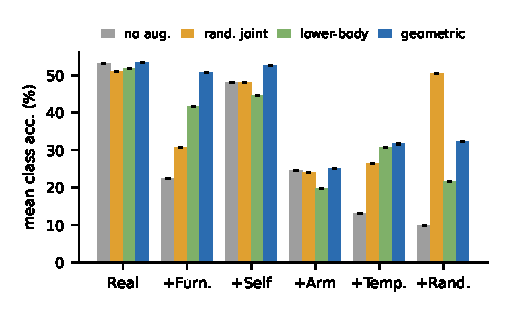
\includegraphics[width=\linewidth]{fig_toyota.pdf}
\caption{Toyota Smarthome mean-class accuracy under added occlusion (mean$\pm$std, 3 seeds).}
\label{fig:toyota}
\end{figure}

On the real Toyota test set (Tab.~\ref{tab:toyota}, Fig.~\ref{fig:toyota}), all schemes are within 1.8 points (51.8--53.6 mean class, 72.5--74.1 top-1).
No augmentation improves on the occlusion already present in these real homes.
Under additional furniture occlusion the unaugmented model collapses ($53.6\rightarrow24.6$).
Geometric training keeps 50.3, against 42.5 for lower-body and 32.3 for random.
Geometric is also best under self-occlusion (52.7).
Combined trades about 2 points on furniture (48.0) for the best result on held-out temporal blocks (36.0 vs.\ 30.3) and near-specialist accuracy on random dropout (49.4 vs.\ 51.3).
Removing a whole arm remains hard for every scheme (19--25 mean class), because 3 of only 13 joints carry most of the hand-object information.

\subsection{Lab-to-home transfer}
\begin{table}[t]
\centering\footnotesize
\setlength{\tabcolsep}{3pt}
\begin{tabular}{@{}lcccc@{}}
\toprule
 & \multicolumn{2}{c}{Raw inputs} & \multicolumn{2}{c}{Harmonized} \\
\cmidrule(lr){2-3}\cmidrule(l){4-5}
Train aug. (NTU) & Top-1 & Mean cls. & Top-1 & Mean cls. \\
\midrule
-- & 15.8 & 17.8 & 23.7$\pm$1.1 & 27.5$\pm$2.9 \\
rand. joint & 11.5 & 17.9 & 19.5$\pm$0.5 & 22.4$\pm$0.5 \\
lower-body (prop.) & 16.3 & 19.4 & 25.2$\pm$2.4 & 26.3$\pm$1.7 \\
geometric (ours) & 15.2 & 19.2 & 22.6$\pm$4.3 & 26.3$\pm$3.5 \\
combined (ours) & -- & -- & 22.1$\pm$1.1 & 26.0$\pm$2.1 \\
\bottomrule
\end{tabular}

\caption{Zero-shot NTU$\rightarrow$Toyota on the 8 shared classes (7{,}520 Toyota clips; chance 12.5\%).
Models are trained on NTU (13 joints); logits are restricted to the shared classes.
Raw: first-frame centering, 1 seed. Harmonized: per-frame root centering and torso scaling, 3 seeds.}
\label{tab:transfer}
\end{table}

We train on NTU with the 13 shared joints and test on all Toyota clips of 8 shared classes (drink, eat, sit down, stand up, read, phone call, laptop$\rightarrow$type, tablet$\rightarrow$phone).
With raw inputs, transfer is near chance for every scheme (Tab.~\ref{tab:transfer}).
Sit down and stand up are almost never recognized (0--13\%) because the NTU models depend on the global pelvis trajectory, which LCR-Net poses lack.
Harmonized normalization lifts mean-class accuracy to 22--28\% for every scheme.
Sit down and stand up rise to 28--39\% and 34--56\%.
Fine-grained hand-object classes stay low (eat 6--10\%, phone call 6--17\%).
Differences between augmentation schemes are within seed noise (std up to 3.5).
Occlusion augmentation does not close the gap, because occlusion is not the dominant one.
The pose source (Kinect depth vs.\ monocular RGB), viewpoint and the scripted-vs.-spontaneous style of the actions matter more.

%====================================================================
\section{Discussion}\label{sec:disc}
\textbf{What transferred to real data.}
(i)~Masking a \emph{fixed} part (our proposal) does not transfer. It helps only on its own test, and real occlusion affects other parts, mostly the hands on Kinect.
(ii)~Geometric occlusion gives the most robust model on structured occlusion in both the lab and real homes, and it slightly beats random masking on real Kinect failures.
(iii)~Adding sparse random dropout (combined) gives the best model on real Kinect failures and on held-out temporal occlusion.
It costs about 1--2 points on structured furniture occlusion in Toyota, so the choice between the two depends on the sensor.
(iv)~Normalization can matter more than augmentation: one centering mismatch removed a whole cue (global motion) and made two classes unrecognizable.

\textbf{What the simulation gets wrong.}
Kinect loses hands mostly through tracking failure at the extremities, not through being hidden behind the torso.
A third realistic source, \emph{extremity dropout}, is not modeled geometrically.
This is why the random component in the combined scheme helps on NTU-Real.
How missing joints are filled matters as much as which joints go missing.

\textbf{Limitations.}
Toyota occlusion results add simulation on top of real data, since Toyota provides no visibility labels.
The transfer study covers only 8 classes and one backbone.
We did not evaluate the cross-view protocols.
Deployment from RGB keypoints (MediaPipe~\cite{lugaresi2019mediapipe}) and edge-hardware latency, both planned in the proposal, were not pursued.

\section{Conclusion}
Occlusion robustness for home action recognition is better trained by modeling \emph{where occlusion comes from} than by masking joints at random or by fixed parts.
A cheap geometric model of furniture and self-occlusion transfers to real occlusion in real homes and does not cost clean accuracy.
Evaluating on real failures shows which assumptions hold: lower-body dropout does not, and sensor dropout of the extremities matters.
Code: \url{https://github.com/KarthikRed2000/Smart-Environment-Action-Recognition}.

\paragraph{Acknowledgements.}
(Portions of) the research in this paper used the NTU RGB+D Action Recognition Dataset made available by the ROSE Lab at the Nanyang Technological University, Singapore.
We use the Toyota Smarthome dataset~\cite{das2019toyota}, provided by Toyota Motor Europe and Inria.
Compute was provided through Google Cloud Platform.

{\small
\bibliographystyle{ieeenat_fullname}
\bibliography{refs}
}
\end{document}
